\section{Results} \label{sec:results}
% focus on the results, not on the analysis
% TODO irgendwie zu kurz, irgendwie keine Information, nochmal überarbeiten

{\color{lightgray}
% intro
We will provide an overview of the Top 10 genes found by the graph algorithm,
which are crucial for understanding the complex interactions within the extended PPI network.


% Presentation of the 10 Genes
To identify the most significant genes, we extracted the top 10 genes with the highest PageRank scores from the list of relevant genes,
as shown in Figure~\ref{fig:03_03_df_pagerank_relevant}.
These genes are not only highly connected within the network but also exhibit a substantial change in gene activity.

\begin{figure}[h]
    \centering
    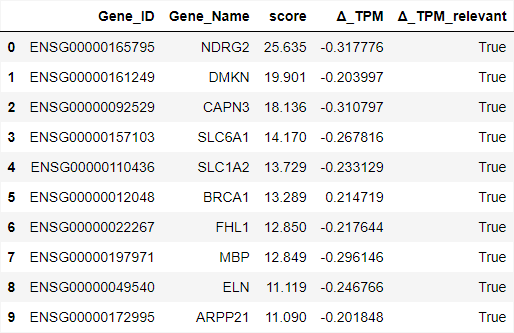
\includegraphics[height=\dfheightdouble]{figures/03_03_df_pagerank_relevant}
    \caption{Top 10 Genes with the highest PageRank scores and a significant change in gene activity}
    \label{fig:03_03_df_pagerank_relevant}
\end{figure}


% Outro
The key findings of this chapter include a list of 10 genes that are likely to be biomarkers for lung cancer.
}